\documentclass{article}
\usepackage{iclr2027_conference,times}
%%%%% NEW MATH DEFINITIONS %%%%%

\usepackage{amsmath,amsfonts,bm}

% Mark sections of captions for referring to divisions of figures
\newcommand{\figleft}{{\em (Left)}}
\newcommand{\figcenter}{{\em (Center)}}
\newcommand{\figright}{{\em (Right)}}
\newcommand{\figtop}{{\em (Top)}}
\newcommand{\figbottom}{{\em (Bottom)}}
\newcommand{\captiona}{{\em (a)}}
\newcommand{\captionb}{{\em (b)}}
\newcommand{\captionc}{{\em (c)}}
\newcommand{\captiond}{{\em (d)}}

% Highlight a newly defined term
\newcommand{\newterm}[1]{{\bf #1}}


% Figure reference, lower-case.
\def\figref#1{figure~\ref{#1}}
% Figure reference, capital. For start of sentence
\def\Figref#1{Figure~\ref{#1}}
\def\twofigref#1#2{figures \ref{#1} and \ref{#2}}
\def\quadfigref#1#2#3#4{figures \ref{#1}, \ref{#2}, \ref{#3} and \ref{#4}}
% Section reference, lower-case.
\def\secref#1{section~\ref{#1}}
% Section reference, capital.
\def\Secref#1{Section~\ref{#1}}
% Reference to two sections.
\def\twosecrefs#1#2{sections \ref{#1} and \ref{#2}}
% Reference to three sections.
\def\secrefs#1#2#3{sections \ref{#1}, \ref{#2} and \ref{#3}}
% Reference to an equation, lower-case.
\def\eqref#1{equation~\ref{#1}}
% Reference to an equation, upper case
\def\Eqref#1{Equation~\ref{#1}}
% A raw reference to an equation---avoid using if possible
\def\plaineqref#1{\ref{#1}}
% Reference to a chapter, lower-case.
\def\chapref#1{chapter~\ref{#1}}
% Reference to an equation, upper case.
\def\Chapref#1{Chapter~\ref{#1}}
% Reference to a range of chapters
\def\rangechapref#1#2{chapters\ref{#1}--\ref{#2}}
% Reference to an algorithm, lower-case.
\def\algref#1{algorithm~\ref{#1}}
% Reference to an algorithm, upper case.
\def\Algref#1{Algorithm~\ref{#1}}
\def\twoalgref#1#2{algorithms \ref{#1} and \ref{#2}}
\def\Twoalgref#1#2{Algorithms \ref{#1} and \ref{#2}}
% Reference to a part, lower case
\def\partref#1{part~\ref{#1}}
% Reference to a part, upper case
\def\Partref#1{Part~\ref{#1}}
\def\twopartref#1#2{parts \ref{#1} and \ref{#2}}

\def\ceil#1{\lceil #1 \rceil}
\def\floor#1{\lfloor #1 \rfloor}
\def\1{\bm{1}}
\newcommand{\train}{\mathcal{D}}
\newcommand{\valid}{\mathcal{D_{\mathrm{valid}}}}
\newcommand{\test}{\mathcal{D_{\mathrm{test}}}}

\def\eps{{\epsilon}}


% Random variables
\def\reta{{\textnormal{$\eta$}}}
\def\ra{{\textnormal{a}}}
\def\rb{{\textnormal{b}}}
\def\rc{{\textnormal{c}}}
\def\rd{{\textnormal{d}}}
\def\re{{\textnormal{e}}}
\def\rf{{\textnormal{f}}}
\def\rg{{\textnormal{g}}}
\def\rh{{\textnormal{h}}}
\def\ri{{\textnormal{i}}}
\def\rj{{\textnormal{j}}}
\def\rk{{\textnormal{k}}}
\def\rl{{\textnormal{l}}}
% rm is already a command, just don't name any random variables m
\def\rn{{\textnormal{n}}}
\def\ro{{\textnormal{o}}}
\def\rp{{\textnormal{p}}}
\def\rq{{\textnormal{q}}}
\def\rr{{\textnormal{r}}}
\def\rs{{\textnormal{s}}}
\def\rt{{\textnormal{t}}}
\def\ru{{\textnormal{u}}}
\def\rv{{\textnormal{v}}}
\def\rw{{\textnormal{w}}}
\def\rx{{\textnormal{x}}}
\def\ry{{\textnormal{y}}}
\def\rz{{\textnormal{z}}}

% Random vectors
\def\rvepsilon{{\mathbf{\epsilon}}}
\def\rvtheta{{\mathbf{\theta}}}
\def\rva{{\mathbf{a}}}
\def\rvb{{\mathbf{b}}}
\def\rvc{{\mathbf{c}}}
\def\rvd{{\mathbf{d}}}
\def\rve{{\mathbf{e}}}
\def\rvf{{\mathbf{f}}}
\def\rvg{{\mathbf{g}}}
\def\rvh{{\mathbf{h}}}
\def\rvu{{\mathbf{i}}}
\def\rvj{{\mathbf{j}}}
\def\rvk{{\mathbf{k}}}
\def\rvl{{\mathbf{l}}}
\def\rvm{{\mathbf{m}}}
\def\rvn{{\mathbf{n}}}
\def\rvo{{\mathbf{o}}}
\def\rvp{{\mathbf{p}}}
\def\rvq{{\mathbf{q}}}
\def\rvr{{\mathbf{r}}}
\def\rvs{{\mathbf{s}}}
\def\rvt{{\mathbf{t}}}
\def\rvu{{\mathbf{u}}}
\def\rvv{{\mathbf{v}}}
\def\rvw{{\mathbf{w}}}
\def\rvx{{\mathbf{x}}}
\def\rvy{{\mathbf{y}}}
\def\rvz{{\mathbf{z}}}

% Elements of random vectors
\def\erva{{\textnormal{a}}}
\def\ervb{{\textnormal{b}}}
\def\ervc{{\textnormal{c}}}
\def\ervd{{\textnormal{d}}}
\def\erve{{\textnormal{e}}}
\def\ervf{{\textnormal{f}}}
\def\ervg{{\textnormal{g}}}
\def\ervh{{\textnormal{h}}}
\def\ervi{{\textnormal{i}}}
\def\ervj{{\textnormal{j}}}
\def\ervk{{\textnormal{k}}}
\def\ervl{{\textnormal{l}}}
\def\ervm{{\textnormal{m}}}
\def\ervn{{\textnormal{n}}}
\def\ervo{{\textnormal{o}}}
\def\ervp{{\textnormal{p}}}
\def\ervq{{\textnormal{q}}}
\def\ervr{{\textnormal{r}}}
\def\ervs{{\textnormal{s}}}
\def\ervt{{\textnormal{t}}}
\def\ervu{{\textnormal{u}}}
\def\ervv{{\textnormal{v}}}
\def\ervw{{\textnormal{w}}}
\def\ervx{{\textnormal{x}}}
\def\ervy{{\textnormal{y}}}
\def\ervz{{\textnormal{z}}}

% Random matrices
\def\rmA{{\mathbf{A}}}
\def\rmB{{\mathbf{B}}}
\def\rmC{{\mathbf{C}}}
\def\rmD{{\mathbf{D}}}
\def\rmE{{\mathbf{E}}}
\def\rmF{{\mathbf{F}}}
\def\rmG{{\mathbf{G}}}
\def\rmH{{\mathbf{H}}}
\def\rmI{{\mathbf{I}}}
\def\rmJ{{\mathbf{J}}}
\def\rmK{{\mathbf{K}}}
\def\rmL{{\mathbf{L}}}
\def\rmM{{\mathbf{M}}}
\def\rmN{{\mathbf{N}}}
\def\rmO{{\mathbf{O}}}
\def\rmP{{\mathbf{P}}}
\def\rmQ{{\mathbf{Q}}}
\def\rmR{{\mathbf{R}}}
\def\rmS{{\mathbf{S}}}
\def\rmT{{\mathbf{T}}}
\def\rmU{{\mathbf{U}}}
\def\rmV{{\mathbf{V}}}
\def\rmW{{\mathbf{W}}}
\def\rmX{{\mathbf{X}}}
\def\rmY{{\mathbf{Y}}}
\def\rmZ{{\mathbf{Z}}}

% Elements of random matrices
\def\ermA{{\textnormal{A}}}
\def\ermB{{\textnormal{B}}}
\def\ermC{{\textnormal{C}}}
\def\ermD{{\textnormal{D}}}
\def\ermE{{\textnormal{E}}}
\def\ermF{{\textnormal{F}}}
\def\ermG{{\textnormal{G}}}
\def\ermH{{\textnormal{H}}}
\def\ermI{{\textnormal{I}}}
\def\ermJ{{\textnormal{J}}}
\def\ermK{{\textnormal{K}}}
\def\ermL{{\textnormal{L}}}
\def\ermM{{\textnormal{M}}}
\def\ermN{{\textnormal{N}}}
\def\ermO{{\textnormal{O}}}
\def\ermP{{\textnormal{P}}}
\def\ermQ{{\textnormal{Q}}}
\def\ermR{{\textnormal{R}}}
\def\ermS{{\textnormal{S}}}
\def\ermT{{\textnormal{T}}}
\def\ermU{{\textnormal{U}}}
\def\ermV{{\textnormal{V}}}
\def\ermW{{\textnormal{W}}}
\def\ermX{{\textnormal{X}}}
\def\ermY{{\textnormal{Y}}}
\def\ermZ{{\textnormal{Z}}}

% Vectors
\def\vzero{{\bm{0}}}
\def\vone{{\bm{1}}}
\def\vmu{{\bm{\mu}}}
\def\vtheta{{\bm{\theta}}}
\def\va{{\bm{a}}}
\def\vb{{\bm{b}}}
\def\vc{{\bm{c}}}
\def\vd{{\bm{d}}}
\def\ve{{\bm{e}}}
\def\vf{{\bm{f}}}
\def\vg{{\bm{g}}}
\def\vh{{\bm{h}}}
\def\vi{{\bm{i}}}
\def\vj{{\bm{j}}}
\def\vk{{\bm{k}}}
\def\vl{{\bm{l}}}
\def\vm{{\bm{m}}}
\def\vn{{\bm{n}}}
\def\vo{{\bm{o}}}
\def\vp{{\bm{p}}}
\def\vq{{\bm{q}}}
\def\vr{{\bm{r}}}
\def\vs{{\bm{s}}}
\def\vt{{\bm{t}}}
\def\vu{{\bm{u}}}
\def\vv{{\bm{v}}}
\def\vw{{\bm{w}}}
\def\vx{{\bm{x}}}
\def\vy{{\bm{y}}}
\def\vz{{\bm{z}}}

% Elements of vectors
\def\evalpha{{\alpha}}
\def\evbeta{{\beta}}
\def\evepsilon{{\epsilon}}
\def\evlambda{{\lambda}}
\def\evomega{{\omega}}
\def\evmu{{\mu}}
\def\evpsi{{\psi}}
\def\evsigma{{\sigma}}
\def\evtheta{{\theta}}
\def\eva{{a}}
\def\evb{{b}}
\def\evc{{c}}
\def\evd{{d}}
\def\eve{{e}}
\def\evf{{f}}
\def\evg{{g}}
\def\evh{{h}}
\def\evi{{i}}
\def\evj{{j}}
\def\evk{{k}}
\def\evl{{l}}
\def\evm{{m}}
\def\evn{{n}}
\def\evo{{o}}
\def\evp{{p}}
\def\evq{{q}}
\def\evr{{r}}
\def\evs{{s}}
\def\evt{{t}}
\def\evu{{u}}
\def\evv{{v}}
\def\evw{{w}}
\def\evx{{x}}
\def\evy{{y}}
\def\evz{{z}}

% Matrix
\def\mA{{\bm{A}}}
\def\mB{{\bm{B}}}
\def\mC{{\bm{C}}}
\def\mD{{\bm{D}}}
\def\mE{{\bm{E}}}
\def\mF{{\bm{F}}}
\def\mG{{\bm{G}}}
\def\mH{{\bm{H}}}
\def\mI{{\bm{I}}}
\def\mJ{{\bm{J}}}
\def\mK{{\bm{K}}}
\def\mL{{\bm{L}}}
\def\mM{{\bm{M}}}
\def\mN{{\bm{N}}}
\def\mO{{\bm{O}}}
\def\mP{{\bm{P}}}
\def\mQ{{\bm{Q}}}
\def\mR{{\bm{R}}}
\def\mS{{\bm{S}}}
\def\mT{{\bm{T}}}
\def\mU{{\bm{U}}}
\def\mV{{\bm{V}}}
\def\mW{{\bm{W}}}
\def\mX{{\bm{X}}}
\def\mY{{\bm{Y}}}
\def\mZ{{\bm{Z}}}
\def\mBeta{{\bm{\beta}}}
\def\mPhi{{\bm{\Phi}}}
\def\mLambda{{\bm{\Lambda}}}
\def\mSigma{{\bm{\Sigma}}}

% Tensor
\DeclareMathAlphabet{\mathsfit}{\encodingdefault}{\sfdefault}{m}{sl}
\SetMathAlphabet{\mathsfit}{bold}{\encodingdefault}{\sfdefault}{bx}{n}
\newcommand{\tens}[1]{\bm{\mathsfit{#1}}}
\def\tA{{\tens{A}}}
\def\tB{{\tens{B}}}
\def\tC{{\tens{C}}}
\def\tD{{\tens{D}}}
\def\tE{{\tens{E}}}
\def\tF{{\tens{F}}}
\def\tG{{\tens{G}}}
\def\tH{{\tens{H}}}
\def\tI{{\tens{I}}}
\def\tJ{{\tens{J}}}
\def\tK{{\tens{K}}}
\def\tL{{\tens{L}}}
\def\tM{{\tens{M}}}
\def\tN{{\tens{N}}}
\def\tO{{\tens{O}}}
\def\tP{{\tens{P}}}
\def\tQ{{\tens{Q}}}
\def\tR{{\tens{R}}}
\def\tS{{\tens{S}}}
\def\tT{{\tens{T}}}
\def\tU{{\tens{U}}}
\def\tV{{\tens{V}}}
\def\tW{{\tens{W}}}
\def\tX{{\tens{X}}}
\def\tY{{\tens{Y}}}
\def\tZ{{\tens{Z}}}


% Graph
\def\gA{{\mathcal{A}}}
\def\gB{{\mathcal{B}}}
\def\gC{{\mathcal{C}}}
\def\gD{{\mathcal{D}}}
\def\gE{{\mathcal{E}}}
\def\gF{{\mathcal{F}}}
\def\gG{{\mathcal{G}}}
\def\gH{{\mathcal{H}}}
\def\gI{{\mathcal{I}}}
\def\gJ{{\mathcal{J}}}
\def\gK{{\mathcal{K}}}
\def\gL{{\mathcal{L}}}
\def\gM{{\mathcal{M}}}
\def\gN{{\mathcal{N}}}
\def\gO{{\mathcal{O}}}
\def\gP{{\mathcal{P}}}
\def\gQ{{\mathcal{Q}}}
\def\gR{{\mathcal{R}}}
\def\gS{{\mathcal{S}}}
\def\gT{{\mathcal{T}}}
\def\gU{{\mathcal{U}}}
\def\gV{{\mathcal{V}}}
\def\gW{{\mathcal{W}}}
\def\gX{{\mathcal{X}}}
\def\gY{{\mathcal{Y}}}
\def\gZ{{\mathcal{Z}}}

% Sets
\def\sA{{\mathbb{A}}}
\def\sB{{\mathbb{B}}}
\def\sC{{\mathbb{C}}}
\def\sD{{\mathbb{D}}}
% Don't use a set called E, because this would be the same as our symbol
% for expectation.
\def\sF{{\mathbb{F}}}
\def\sG{{\mathbb{G}}}
\def\sH{{\mathbb{H}}}
\def\sI{{\mathbb{I}}}
\def\sJ{{\mathbb{J}}}
\def\sK{{\mathbb{K}}}
\def\sL{{\mathbb{L}}}
\def\sM{{\mathbb{M}}}
\def\sN{{\mathbb{N}}}
\def\sO{{\mathbb{O}}}
\def\sP{{\mathbb{P}}}
\def\sQ{{\mathbb{Q}}}
\def\sR{{\mathbb{R}}}
\def\sS{{\mathbb{S}}}
\def\sT{{\mathbb{T}}}
\def\sU{{\mathbb{U}}}
\def\sV{{\mathbb{V}}}
\def\sW{{\mathbb{W}}}
\def\sX{{\mathbb{X}}}
\def\sY{{\mathbb{Y}}}
\def\sZ{{\mathbb{Z}}}

% Entries of a matrix
\def\emLambda{{\Lambda}}
\def\emA{{A}}
\def\emB{{B}}
\def\emC{{C}}
\def\emD{{D}}
\def\emE{{E}}
\def\emF{{F}}
\def\emG{{G}}
\def\emH{{H}}
\def\emI{{I}}
\def\emJ{{J}}
\def\emK{{K}}
\def\emL{{L}}
\def\emM{{M}}
\def\emN{{N}}
\def\emO{{O}}
\def\emP{{P}}
\def\emQ{{Q}}
\def\emR{{R}}
\def\emS{{S}}
\def\emT{{T}}
\def\emU{{U}}
\def\emV{{V}}
\def\emW{{W}}
\def\emX{{X}}
\def\emY{{Y}}
\def\emZ{{Z}}
\def\emSigma{{\Sigma}}

% entries of a tensor
% Same font as tensor, without \bm wrapper
\newcommand{\etens}[1]{\mathsfit{#1}}
\def\etLambda{{\etens{\Lambda}}}
\def\etA{{\etens{A}}}
\def\etB{{\etens{B}}}
\def\etC{{\etens{C}}}
\def\etD{{\etens{D}}}
\def\etE{{\etens{E}}}
\def\etF{{\etens{F}}}
\def\etG{{\etens{G}}}
\def\etH{{\etens{H}}}
\def\etI{{\etens{I}}}
\def\etJ{{\etens{J}}}
\def\etK{{\etens{K}}}
\def\etL{{\etens{L}}}
\def\etM{{\etens{M}}}
\def\etN{{\etens{N}}}
\def\etO{{\etens{O}}}
\def\etP{{\etens{P}}}
\def\etQ{{\etens{Q}}}
\def\etR{{\etens{R}}}
\def\etS{{\etens{S}}}
\def\etT{{\etens{T}}}
\def\etU{{\etens{U}}}
\def\etV{{\etens{V}}}
\def\etW{{\etens{W}}}
\def\etX{{\etens{X}}}
\def\etY{{\etens{Y}}}
\def\etZ{{\etens{Z}}}

% The true underlying data generating distribution
\newcommand{\pdata}{p_{\rm{data}}}
% The empirical distribution defined by the training set
\newcommand{\ptrain}{\hat{p}_{\rm{data}}}
\newcommand{\Ptrain}{\hat{P}_{\rm{data}}}
% The model distribution
\newcommand{\pmodel}{p_{\rm{model}}}
\newcommand{\Pmodel}{P_{\rm{model}}}
\newcommand{\ptildemodel}{\tilde{p}_{\rm{model}}}
% Stochastic autoencoder distributions
\newcommand{\pencode}{p_{\rm{encoder}}}
\newcommand{\pdecode}{p_{\rm{decoder}}}
\newcommand{\precons}{p_{\rm{reconstruct}}}

\newcommand{\laplace}{\mathrm{Laplace}} % Laplace distribution

\newcommand{\E}{\mathbb{E}}
\newcommand{\Ls}{\mathcal{L}}
\newcommand{\R}{\mathbb{R}}
\newcommand{\emp}{\tilde{p}}
\newcommand{\lr}{\alpha}
\newcommand{\reg}{\lambda}
\newcommand{\rect}{\mathrm{rectifier}}
\newcommand{\softmax}{\mathrm{softmax}}
\newcommand{\sigmoid}{\sigma}
\newcommand{\softplus}{\zeta}
\newcommand{\KL}{D_{\mathrm{KL}}}
\newcommand{\Var}{\mathrm{Var}}
\newcommand{\standarderror}{\mathrm{SE}}
\newcommand{\Cov}{\mathrm{Cov}}
% Wolfram Mathworld says $L^2$ is for function spaces and $\ell^2$ is for vectors
% But then they seem to use $L^2$ for vectors throughout the site, and so does
% wikipedia.
\newcommand{\normlzero}{L^0}
\newcommand{\normlone}{L^1}
\newcommand{\normltwo}{L^2}
\newcommand{\normlp}{L^p}
\newcommand{\normmax}{L^\infty}

\newcommand{\parents}{Pa} % See usage in notation.tex. Chosen to match Daphne's book.

\DeclareMathOperator*{\argmax}{arg\,max}
\DeclareMathOperator*{\argmin}{arg\,min}

\DeclareMathOperator{\sign}{sign}
\DeclareMathOperator{\Tr}{Tr}
\let\ab\allowbreak


\usepackage{amsmath}
\usepackage{amssymb}
\usepackage{amsthm}
\usepackage{booktabs}
\usepackage{graphicx}
\usepackage{microtype}
\usepackage{multirow}
\usepackage{algorithm}
\usepackage{algpseudocode}
\usepackage[section]{placeins}
\usepackage{url}
\usepackage{hyperref}

\newtheorem{theorem}{Theorem}
\newtheorem{proposition}[theorem]{Proposition}
\newtheorem{corollary}[theorem]{Corollary}
\theoremstyle{definition}
\newtheorem{definition}{Definition}
\theoremstyle{remark}
\newtheorem{remark}{Remark}

\newcommand{\Fsig}{F_{\sigma}}
\newcommand{\sgnx}{\operatorname{sign}}
\newcommand{\Ex}{\mathbb{E}}
\newcommand{\Rl}{\mathbb{R}}
\newcommand{\RSSx}{\mathrm{RSS}}
\newcommand{\dof}{\mathrm{df}}
\newcommand{\flr}{\mathrm{floor}}

\title{Six Requirements for Inference-Time\\Self-Iterating Models: Representation,\\Uncertainty, and Local Credit}

\author{Anonymous authors\\
Paper under double-blind review}

\begin{document}
\maketitle

\begin{abstract}
Inference-time self-iteration lets a model run an iterative learner on its context before it answers.
For multi-branch in-context relations---how \emph{different} two items are along an attribute the model was never trained on, or compressive phase retrieval---a lifted inner loop (per-example global inversion, multipliers, local least squares) provably reaches what test-time training's gradient update, fixed-feature closed-form heads and additional layers cannot.
Whether a pretrained model can host such a loop depends on its representation.
We prove six requirements.
Two concern the \emph{representation} and hold for every learner: the task must be decodable from the base, which sets an explicit error floor $\flr(\nu)$ in terms of the base's undecodable fraction $\nu$ (R1), and it must be identifiable from the context, which ties the task dimension to the context size and calls for posterior mixtures near the threshold (R2).
Two concern \emph{uncertainty}: inversion and readout must be consistent with the base's residual noise (R3), and in-context noise estimates must be corrected for degrees of freedom (R4).
Two concern \emph{local credit}: the multiplier leak must vanish on exactly decodable bases and grow with the noise (R5), and the knobs that control branch changes must be selected, not trained by backpropagation (R6).
R1 and R2 give measurable diagnostics of a base.
On word vectors (GloVe), a molecular graph network (GINE) and an image code (PCA), which satisfy them, the matched self-iterating learner beats gradient test-time training, quadratic closed-form heads and Transformers, with a second-seed replication and paired tests; on a base that violates decodability (MiniLM word vectors) every learner, including an oracle probe, stays above the proven floor.
\end{abstract}

\section{Introduction}

Test-time training (TTT) turns a layer's hidden state into a learner that is updated on the current context \citep{sun2023ttt,sun2024ttt}; fast-weight programmers and test-time regression place many sequence models in the same design space, with inner updates that are single gradient steps or closed-form regressions \citep{schlag2021fastweights,wang2026ttr}.
The natural next step is \emph{self-iteration}: let the inner learner run an iterative solver on the context before answering.
Self-iteration is only as good as the representation it iterates on.
This paper asks the question that decides whether it can be used: \emph{what must the pretrained base satisfy, and what must the self-iterating learner satisfy on that base?}

We answer for multi-branch in-context relations.
When a context shows pairs of items with \emph{how different} they are along an unseen attribute, the label is $y=|u^\top(k_a-k_b)+\varepsilon|$, a sign-lost function of a task-specific direction plus the part of the attribute the base does not encode; phase retrieval has the same form.

\paragraph{Why self-iteration.}
On such relations a lifted inner loop---each context example gets an activity that is inverted globally in one dimension, multipliers coordinate the activities with a shared memory, and the memory is refit by local least squares, a predictive-coding augmented Lagrangian \citep{seely2026pcalm}---solves tasks that are out of reach for fixed-feature closed-form heads (which have a sample-independent floor, Theorem~\ref{thm:features}), for correlational gradient updates, and for added layers (Section~\ref{sec:why}).

\paragraph{Six requirements.}
\emph{Representation} (Section~\ref{sec:base}), provable for every learner:
(R1) \emph{decodability}---if a fraction $\nu$ of the attribute is not decodable from the base, every learner has normalized error at least $\flr(\nu)$, with $\flr(0.5)=0.77$, and deployment directions outside the keys' span add to $\nu$;
(R2) \emph{identifiability}---fewer context examples than task dimensions leave the task unidentified for every learner, and near the threshold the Bayes predictor is a posterior mixture.
\emph{Uncertainty} and \emph{local credit} (Section~\ref{sec:learner}), for the self-iterating learner on a base with $\nu>0$:
(R3) inversion and readout consistent with residual noise inside the nonlinearity;
(R4) degrees-of-freedom-corrected in-context noise estimates;
(R5) a multiplier leak that vanishes when $\nu=0$ and grows with $\nu$;
(R6) derivative-free selection of branch-controlling solver knobs, because backpropagation through the solver omits exactly the branch-change term.

\paragraph{Evidence.}
Each theorem is confirmed quantitatively on controlled bases (Section~\ref{sec:verify}).
The base diagnostics then predict the outcome on real bases (Section~\ref{sec:real}): GloVe word vectors, a GINE molecular encoder and a PCA image code satisfy R1--R2, and the self-iterating learner that satisfies R3--R6 is the best inner loop on all of them; MiniLM word vectors violate R1, and every learner, including an oracle probe trained on all labels, stays above the proven floor.

\section{Setting}
\label{sec:setting}

\paragraph{Base, TTT layer, inner loop.}
A pretrained base maps an input $x$ to an embedding; a TTT layer projects it to keys $k=\theta(x)\in\Rl^d$.
Given a context $D=\{(k_i,y_i)\}_{i=1}^n$ ($K\in\Rl^{n\times d}$), an inner loop computes a memory $w=\mathcal A(K,y)$ and answers a query by $\hat y_q=R(k_q^\top w)$; $\theta$, solver scalars and readout are trained on training tasks.
We compare inner loops with identical keys, data and outer training:
TTT gradient updates (official single pass with one step per mini-batch; full-batch descent with a learned step) \citep{sun2024ttt};
closed-form heads (ridge on keys; ridge on quadratic features $\mathrm{vec}(kk^\top)$ predicting $y^2$, which contains the exact class $|k^\top w|^2$) \citep{bertinetto2019r2d2,wang2026ttr};
a Transformer trained in context (additional layers) \citep{garg2022icl};
and the lifted self-iterating loop.

\paragraph{Multi-branch relations on a base.}
An attribute of an item decomposes as $A(x)=u^\top k(x)+\epsilon(x)$, where $\epsilon$ is the part not linearly decodable from the base.
With standardized attributes, the \emph{base noise ratio} of the task is $\nu=\mathrm{Var}(\epsilon)/\mathrm{Var}(A)=1-R^2$.
The pair relation is
\begin{equation}
y=|m+e|,\qquad m=u^\top(k_a-k_b)\sim\mathcal N(0,2(1-\nu)),\quad e=\epsilon_a-\epsilon_b\sim\mathcal N(0,2\nu),
\label{eq:model}
\end{equation}
with the residual \emph{inside} the nonlinearity; compressive phase retrieval $y=|a^\top x|$ on an image code has the same form with $e=a^\top x_\perp$ the energy outside the code.
We write $\Fsig(m)=\Ex|m+e|=\sigma\sqrt{2/\pi}e^{-m^2/2\sigma^2}+m\,\mathrm{erf}(m/\sqrt2\sigma)$, $\sigma^2=\mathrm{Var}(e)$.

\paragraph{The lifted inner loop.}
With an activity $s_i$ per example, local loss $\ell_y(s)=(|s|-y)^2$, coupling $s=Kw$, multipliers $\lambda$, penalty $\rho$ and leak $v\geq0$:
\begin{align}
s_i&\leftarrow \operatorname*{arg\,min}_s\ \ell_{y_i}(s)+\tfrac{\rho}{2}(s-a_i)^2,\quad a_i=k_i^\top w-\lambda_i/\rho, \label{eq:act}\\
\lambda&\leftarrow(\lambda+\rho(s-Kw))/(1+\rho v),\label{eq:mult}\\
w&\leftarrow(K^\top K+\mu I)^{-1}K^\top(s+\lambda/\rho). \label{eq:ls}
\end{align}
The activity step is a one-dimensional global minimization with two closed-form branch candidates; the parameter step uses no chain rule.
With $v=0$, fixed $\rho$, exact local steps and $\mu\to0$ the iteration is proximal Douglas--Rachford on the lifted problem (Appendix~\ref{app:dr}), in the family of HIO/DR phase-retrieval methods \citep{fienup1982phase,bauschke2002phase}.

\section{Why self-iteration}
\label{sec:why}

On an exactly decodable base ($\nu=0$) the question is which inner loop can learn the relation at all.
We use the multi-branch family $y=g(u^\top x)$, $g=\mathrm{He}_3/\sqrt6$, $x\sim\mathcal N(0,I_d)$, $u$ uniform on the sphere (three preimage branches, information exponent~3).

\begin{theorem}[Fixed-feature floor]
\label{thm:features}
For any $u$-independent features $\varphi:\Rl^d\to\Rl^M$, $M\geq d$, and any coefficients $a(u)$,
$\Ex_u\Ex_x\big(g(u^\top x)-a(u)^\top\varphi(x)\big)^2\geq \frac{d-1}{d+2}\big(1-\frac{(M-d)_+}{N_3}\big)$, where $N_3=\binom{d+2}{3}-d$.
\end{theorem}

The bound holds with unlimited context and an oracle fit, so it covers ridge, random-feature and kernel heads (Appendix~\ref{app:features}).
Gradient credit is correlational: the one-pass online update of official TTT needs $n\gtrsim d^{3/2}$ samples \citep{benarous2021online,damian2023smoothing}, while full-batch reuse helps \citep{dandi2024reuse,lee2024neural}.
The lifted activity step is a nonlinear label transformation with nonzero first Hermite coefficient, so its first parameter step already has a dimension-free overlap with $u$; multipliers break self-consistent wrong branch assignments, because at a block-stationary state with residual $r_0$ they tilt the energy gap to a legal competitor as $\Delta-t\rho\kappa$ (Appendix~\ref{app:escape}).

\begin{table}[t]
\caption{\textbf{Why self-iteration} ($\nu=0$). Left: success rate (query MSE $<0.05$) at $n=4d$, 64 tasks per cell. Right: end-to-end TTT layer ($d=32$; 64-dim observations with unknown 32-dim signal subspace), success at $n=4d$ (two seeds: 0.90, 0.90) and overlap of the learned keys with the signal subspace.}
\label{tab:exact}
\centering\small
\begin{tabular}{lccccc}
\toprule
Inner loop / head & $d=16$ & 32 & 64 & 128 & 256\\
\midrule
Lifted self-iteration (1 start) & 0.94 & 0.94 & 0.95 & \textbf{1.00} & \textbf{1.00}\\
Backprop, Adam ($64\times3$ starts) & 1.00 & 0.83 & 0.34 & 0.00 & 0.00\\
Backprop, Levenberg--Marquardt (64) & 0.94 & 0.55 & 0.02 & 0.00 & 0.00\\
Random features / RBF / cubic kernel & 0.00 & 0.00 & 0.00 & 0.00 & 0.00\\
Additional layer (2-layer MLP) & 0.00 & 0.00 & 0.00 & 0.00 & 0.00\\
\bottomrule
\end{tabular}
\hfill
\begin{tabular}{lcc}
\toprule
TTT inner loop & success & overlap\\
\midrule
Lifted self-iteration & \textbf{0.90} & \textbf{0.999}\\
official GD & 0.00 & 0.51\\
full-batch GD (30/150 steps) & 0.00 & 0.49\\
closed-form ridge & 0.00 & 0.42\\
Transformer (30k steps) & 0.00 & --\\
\bottomrule
\end{tabular}
\end{table}

Table~\ref{tab:exact}: the lifted loop's sample threshold is $n^\star\approx3$--$4d$ for $d$ from 32 to 256 (single-start full-batch backpropagation needs $16$--$24d$); closed-form heads sit at the floor of Theorem~\ref{thm:features} ($0.957$ measured, $0.966$ predicted at $d=128$, $M=4096$); inside a trained TTT layer the outer loop learns the signal subspace through the lifted loop and through no other inner loop.
For i.i.d.\ Gaussian single-index problems, message passing is a strong alternative \citep{rangan2011gamp}; our comparison is among inner loops a TTT layer can host.

\section{Representation: requirements that hold for every learner}
\label{sec:base}

A \emph{learner} is any map from the context and a query key to a prediction, with any number of iterations; query items are fresh draws.
NMSE is the mean squared error divided by $\mathrm{Var}(y)$.

\begin{theorem}[R1: decodable representation]
\label{thm:b1}
Under \eqref{eq:model} with base noise ratio $\nu\in(0,1)$:
(a) every learner has $\mathrm{NMSE}\geq\flr(\nu):=\Ex[\mathrm{Var}(y\mid m)]/\mathrm{Var}(y)$, where $\mathrm{Var}(y\mid m)=m^2+\sigma^2-\Fsig(m)^2>0$; $\flr$ increases from $\flr(0)=0$ to $\flr(1)=1$ (numerically $\flr(0.06)=0.14$, $\flr(0.2)=0.40$, $\flr(0.3)=0.55$, $\flr(0.5)=0.77$);
(b) every learner's context carries information $I(u;D)\leq n\,C(\nu)$ about the task direction, with $C(\nu)\leq\tfrac12\log(1/\nu)$ nats per example; by Fano's inequality, recovering $u$ to within a $\delta$-packing of the unit sphere with error probability at most $P_e$ requires $n\geq\big((1-P_e)(d-1)\log(1/\delta)-\log2\big)/C(\nu)$.
For Gaussian inputs the sign loss reduces the per-example information from $0.347$ (unsigned channel) to $0.107$ nats at $\nu=0.5$.
\end{theorem}

Part (a) holds even for a learner told $u$; it is the price of the base, not of the learner.
A base with $\flr(\nu)$ close to one supports no useful inference-time learning of this relation by any method.

\begin{corollary}[R1, coverage]
\label{cor:b2}
If inputs are isotropic Gaussian, keys are an orthogonal projection $k=Px$, and a deployment direction $u$ has a component $u_\perp$ outside $\mathrm{range}(P)$, then every learner that sees only keys faces Theorem~\ref{thm:b1} with the effective noise ratio $\nu_{\mathrm{eff}}=\nu+(1-\nu)\|u_\perp\|^2/\|u\|^2$.
\end{corollary}

\begin{proposition}[R2: identifiability]
\label{prop:b3}
(a) If $n<d$, for every sign pattern the set of directions consistent with a noiseless context is an affine subspace of dimension at least $d-n$; under a prior with a density, every learner has strictly positive risk. For $u\sim\mathcal N(0,d^{-1}I)$ and $k\sim\mathcal N(0,I)$, every learner---even one told the signs of all $k_i^\top u$---has $\mathrm{NMSE}\geq1-n/d$.
(b) For $n\leq2d-2$, $w\mapsto|Kw|$ is not injective modulo sign for any $K$, so no learner recovers every direction; for $n\geq2d-1$ it is injective for generic $K$ \citep{balan2006phase}.
\end{proposition}

R1--R2 are properties of the base and the deployment protocol.
They are measurable: $\nu$ is one minus the $R^2$ of a linear probe from the base, and $d$ is the key dimension.

\section{Uncertainty and local credit: requirements for the self-iterating learner}
\label{sec:learner}

On a base with $\nu>0$ the lifted loop of Section~\ref{sec:why}, designed for $\nu=0$, must be adapted.
The following conditions are proved in Appendix~\ref{app:proofs}; $k\sim\mathcal N(0,I)$ and $\|w^\star\|=1$.

\begin{theorem}[R3: consistent inversion and readout]
\label{thm:l1}
Let $\sigma>0$ and $c_\sigma=\Ex[(\Fsig(m)-|m|)|m|]$ with $m\sim\mathcal N(0,1)$.
(a) Every fixed point of \eqref{eq:act}--\eqref{eq:ls} with $v=0$ and $k_i^\top w\neq0$ is a stationary point of $\hat R_n(w)=\sum_i(|k_i^\top w|-y_i)^2+\tfrac{\rho\mu}{2}\|w\|^2$.
(b) The population risk $R(w)=\Ex(|k^\top w|-y)^2$ has $\nabla R(w^\star)=-2c_\sigma w^\star\neq0$ and is minimized along $\{\alpha w^\star\}$ at $\alpha^\star=1+c_\sigma>1$.
(c) $\Ex[y\mid k]=\Fsig(k^\top w^\star)$ and $\Fsig(0)=\sigma\sqrt{2/\pi}>0$, so a readout $|k^\top w|$ is never Bayes-optimal.
(d) The posterior inversion $T_\tau(y,a)=y\tanh(ya/\tau)$ satisfies $\Ex[T_{\sigma^2}(y,m)\mid k]=m$, so $w^\star$ solves the population fixed-point equation of $w\leftarrow\mathrm{LS}(K,T_{\sigma^2}(y,Kw))$; for $\tau\to0$ the identity fails.
\end{theorem}

The implemented activity step averages the two branch candidates of \eqref{eq:act} with Gibbs weights at temperature $\tau$; it equals $\tfrac{\rho a}{2+\rho}+\tfrac{2y}{2+\rho}\tanh\!\big(\tfrac{2\rho ya}{(2+\rho)\tau}\big)$ and tends to $T_{\sigma^2}$ as $\rho\to0$ with $\tau/\rho=\sigma^2$.

\begin{theorem}[R5: noise-dependent multiplier leak]
\label{thm:l2}
With hard inversion and leak $v\geq0$:
(a) the fixed points are exactly the self-consistent branch assignments $b\in\{\pm1\}^n$ with $w=\arg\min_w\sum_i(k_i^\top w-b_iy_i)^2+\mu_v\|w\|^2$, $\mu_v=\tfrac{\rho\mu}{2}(1+\tfrac{2v}{1+\rho v})$---the multiplier decides which fixed point is reached, not the set of fixed points;
(b) at a block-stationary state with residual $r_0$ and a competitor with gap $\Delta>0$ and tilt $\kappa>0$, the gap after $t$ steps is $\Delta-\kappa c_t$, $c_t=\rho\sum_{j=1}^t(1+\rho v)^{-j}$; for $v=0$ every such state is left, for $v>0$ exactly those with $\Delta<\kappa/v$;
(c) for a fixed correct assignment, prior $w^\star\sim\mathcal N(0,d^{-1}I)$ and lifted noise of variance $\sigma^2$, the MSE-optimal ridge is $\mu^\star=d\sigma^2$.
\end{theorem}

So $v$ must vanish at $\nu=0$ (escape from barriers of any height) and grow with the base noise (regularization); we set the slack variance from the in-context noise estimate, $v=g\hat r^2$.

\begin{proposition}[R4: unbiased in-context noise estimate]
\label{prop:l3}
For a linear smoother $H=K(K^\top K+\mu I)^{-1}K^\top$ and targets $t=Kw^\star+\xi$, $\mathrm{Cov}(\xi)=\sigma^2I$:
$\Ex\,\RSSx=\|(I-H)Kw^\star\|^2+\sigma^2(n-2\,\mathrm{tr}H+\mathrm{tr}H^2)$; for $\mu\to0$, $\Ex[\RSSx/n]=\sigma^2(1-d/n)$ and $\Ex[\RSSx/(n-d)]=\sigma^2$.
With $v=g\,\RSSx/n$ the loop has positive feedback: smaller $v$ lowers $\mu_v$, raises $\dof=\mathrm{tr}H$ and lowers $\Ex\,\RSSx/n$.
\end{proposition}

\begin{proposition}[R2, learner side: posterior mixtures]
\label{prop:l4}
If the posterior over memories is $\pi\delta_{w_1}+(1-\pi)\delta_{w_2}$ with $w_1\neq\pm w_2$ and $F$ is strictly increasing in $|m|$, then for almost every query $\Delta(k)=F(k^\top w_1)-F(k^\top w_2)\neq0$, and the point predictor $F(k^\top w_j)$ has excess risk $(1-\pi)^2\Delta^2$ or $\pi^2\Delta^2$ over the Bayes mixture.
\end{proposition}

\begin{theorem}[R6: branch-controlling knobs must be selected]
\label{thm:l5}
Let $w_K(\phi;D)$ be the output of $K$ iterations with hard inversion, $\phi$ a solver knob ($\rho$, $v$ or a temperature scale), $L(\phi)=\Ex_D\,\ell(w_K(\phi;D))$ the outer loss, and suppose the branch pattern partitions task space into regions whose boundary $\Gamma(\phi)$ moves smoothly with normal velocity $V$, with $\ell\circ w_K$ smooth inside each region. Then
\begin{equation}
L'(\phi)=\underbrace{\Ex_D\big[\partial_\phi\,\ell(w_K(\phi;D))\big]}_{\text{backpropagation through the solver}}+\underbrace{\int_{\Gamma(\phi)}[\ell]_\Gamma\,V\,p\,dS}_{\text{change of the branch reached}}.
\end{equation}
With a Gibbs temperature $\tau>0$ the pathwise derivative is exact but concentrates with magnitude $O(1/\tau)$ in bands of width $O(\tau)$ around $\Gamma$. For $v=g\hat r^2$ every derivative with respect to $g$ carries a factor $\hat r_t^2$ and vanishes on noiseless training tasks.
\end{theorem}

Backpropagation therefore cannot tune the knobs whose job is to change branches, nor transfer a leak learned on low-noise training tasks to a noisier deployment; in the TTT layer of Section~\ref{sec:why}, a learned $\rho$ grows from 1 to 219 and success falls from 90\% to 0\%.
The knobs are selected on training data from the deployment regime, and their per-task adaptation comes from in-context statistics (R4).

\paragraph{The learner and its matching rule.}
Algorithm~\ref{alg:learner} implements R2--R6.
Its members differ only in the leak scale $g$: the exact member ($\tau,v\to0$), and noise-calibrated members $g\in\{1,10\}$.
Theorems~\ref{thm:l1} and \ref{thm:l2} predict the matching: $\nu=0$ calls for the exact member, small $\nu$ for a weak leak, larger $\nu$ for a strong leak, and a context near $2d$ for mixtures.

\begin{algorithm}[t]
\caption{Self-iterating inner loop satisfying R2--R6 (R2 through the chain mixture) (per context; $R$ chains)}
\label{alg:learner}
\begin{algorithmic}[1]
\Require keys $K$, targets $y$; $\rho=1$; outer-trained $\mu,c,p,s_r,a_0,a_1$; leak scale $g$ selected on training data (R6)
\State $\dof\gets\mathrm{tr}\big((K^\top K+\mu I)^{-1}K^\top K\big)$
\For{chain $r=1,\dots,R$ from a random $w$ and $\lambda=0$}
\For{$t=1,\dots,T$}
\State $u\gets Kw$;\quad $\hat r^2\gets\frac{1}{n-\dof}\sum_i(y_i-|u_i|)^2$ \Comment{R4}
\State $s\gets$ Gibbs average of the two minimizers of \eqref{eq:act} at $a=u-\lambda/\rho$, temperature $c\,\hat r^2$ \Comment{R3}
\State $\lambda\gets(\lambda+\rho(s-u))/(1+\rho g\hat r^2)$ \Comment{R5}
\State $w\gets(K^\top K+(\mu+p)I)^{-1}\big(K^\top(s+\lambda/\rho)+p\,w\big)$ \Comment{proximal least squares}
\EndFor
\State $\hat y_q^{(r)}\gets a_0F_{\sqrt{s_r}\hat r}(k_q^\top w)+a_1$;\quad $\omega_r\propto\exp(-\tfrac n2\hat r_r^2/\min_{r'}\hat r_{r'}^2)$ \Comment{R3, R2}
\EndFor
\State \Return $\sum_r\omega_r\hat y_q^{(r)}$
\end{algorithmic}
\end{algorithm}

\section{Mechanism experiments: every prediction against its measurement}
\label{sec:mech}

Each theorem makes a numerical prediction that can be checked in seconds with true keys and exact arithmetic (float64, 64--512 tasks per point). Table~\ref{tab:mech} and Figure~\ref{fig:mech} put every prediction next to its measurement.

\begin{table}[t]
\caption{\textbf{Mechanism experiments.} Every prediction next to its measurement (true keys, float64).}
\label{tab:mech}
\centering\small
\resizebox{\linewidth}{!}{%
\begin{tabular}{llll}
\toprule
Claim & Setting & Predicted & Measured\\
\midrule
Theorem~\ref{thm:features} is tight at $M=d$ & $d=8/16/32/64$, optimal features & .700/.833/.912/.955 & .697/.831/.914/.954\\
R1: the Bayes oracle sits on $\flr(\nu)$ & $\nu=0.1/0.3/0.5$ & .223/.550/.776 & .224/.552/.778\\
R1: no learner goes below $\flr(\nu)$ & $\nu\in[0.05,0.6]$, four learners & ratio $\geq1$ & minimum ratio 1.04\\
R2: $\mathrm{NMSE}\geq1-n/d$ for $n<d$ & $n/d=0.5/0.75$, signs revealed & $\geq$ .50/.25 & .75/.45\\
R3: ERM inflation $\alpha^\star=1+c_\sigma$ & $\sigma=0.2/0.5/0.8$, $n=64d$ & 1.0017/1.0232/1.0797 & 1.0025/1.0246/1.0862\\
R5: fixed point $=$ ridge$(\mu_v)$ & $v\in\{0,\dots,10\}$, converged tasks & 0 & $\leq1.2\times10^{-15}$\\
\bottomrule
\end{tabular}}
\end{table}

\begin{figure}[t]
\centering
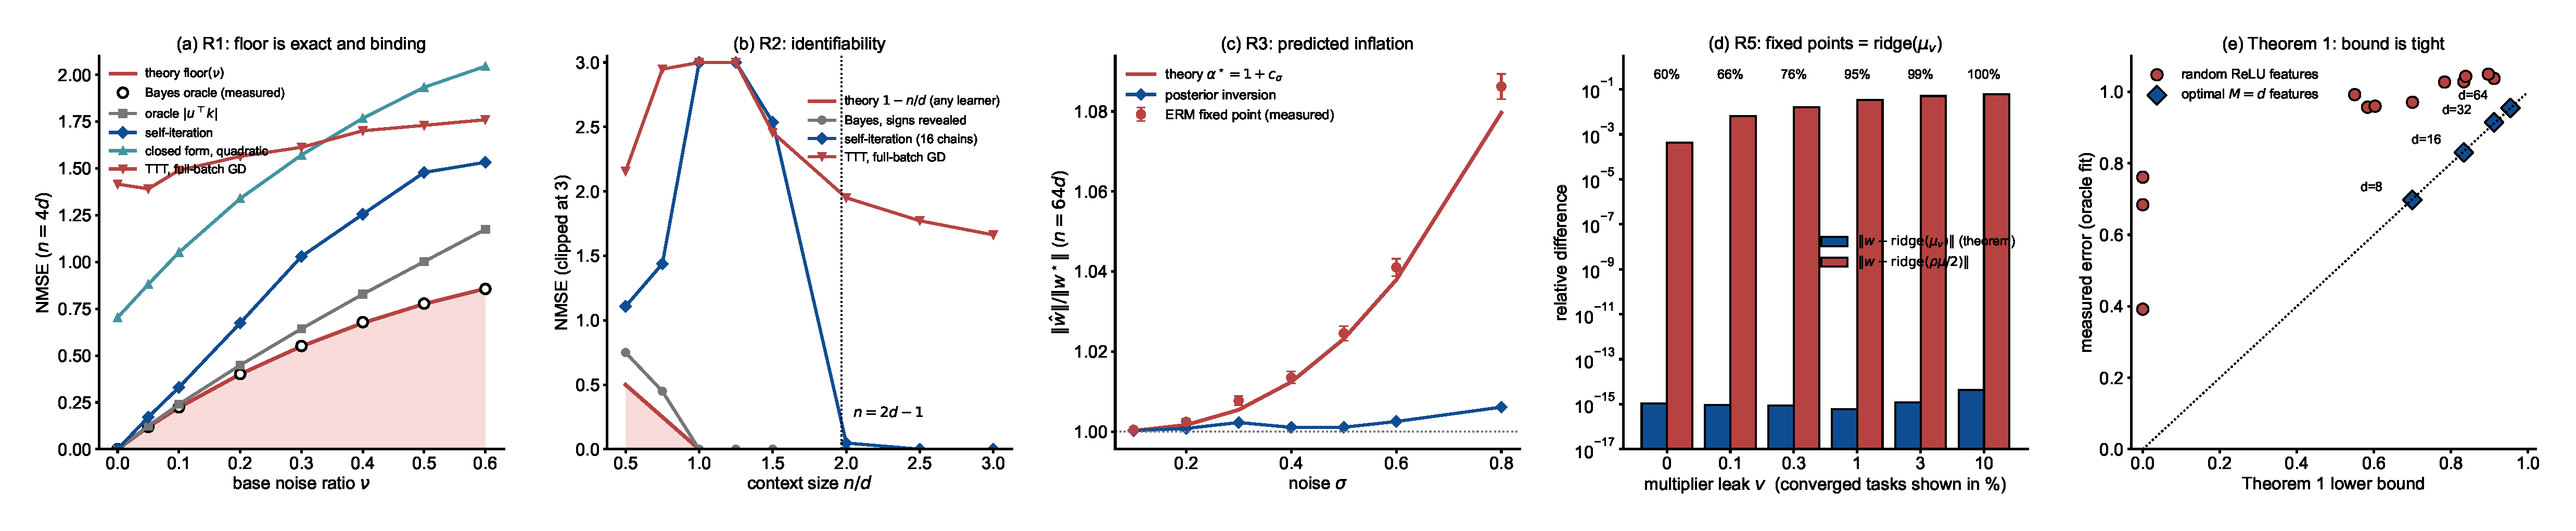
\includegraphics[width=\linewidth]{figures/fig_mechanisms.pdf}
\caption{\textbf{Mechanism experiments.}
(a) R1: on bases with known $\nu$ the Bayes oracle $F_s(u^\top k)$ lies on the theoretical floor (largest deviation 0.004); an oracle $|u^\top k|$ probe, self-iteration, the quadratic closed form and TTT gradient updates all stay above it ($n=4d$, $d=16$).
(b) R2: noiseless contexts; even the Bayes predictor told every sign cannot beat $1-n/d$ below $n=d$; self-iteration (16 chains) solves from $n\approx2d$ (0.048 at $2d$, 0 from $2.5d$), full-batch gradient updates do not.
(c) R3: norm of the ERM fixed point started at $w^\star$ (mean $\pm2$ s.e., 128 tasks, $n=64d$) follows $\alpha^\star(\sigma)$; posterior inversion stays at 1; the remaining excess shrinks with $n$.
(d) R5: at every converged fixed point of the leaky iteration, $w$ equals ridge regression with $\mu_v$ to machine precision, while the unleaked ridge differs by up to 6\%; the percentage of tasks that converge rises from 60\% ($v=0$) to 100\% ($v=10$), since the leak removes limit cycles of the nonconvex iteration.
(e) Theorem~\ref{thm:features}: with the optimal $M=d$ features $x_i(\|x\|^2-d-2)$ the oracle-fit error equals the bound; random ReLU features stay above it.}
\label{fig:mech}
\end{figure}

\paragraph{What the checks establish.}
The floor of R1 is not an upper estimate: the Bayes oracle attains it, so any learner on a base with $\nu=0.5$ is limited to NMSE $\geq0.78$, whatever it iterates.
The R2 bound holds with every sign revealed, so it binds every learner that sees less.
The fixed-point theorem of R5 is exact, and it explains a second effect of the leak visible in (d): beyond regularizing, it turns cycling nonconvex iterations into convergent ones.
The ERM inflation of R3 and the tightness of Theorem~\ref{thm:features} are matched to three decimals.

\section{Verification on controlled bases}
\label{sec:verify}

We verify the learner conditions on controlled bases with known $\nu$ and true keys ($d=32$, 512 tasks per cell, float64; Figure~\ref{fig:controlled}).

\begin{figure}[t]
\centering
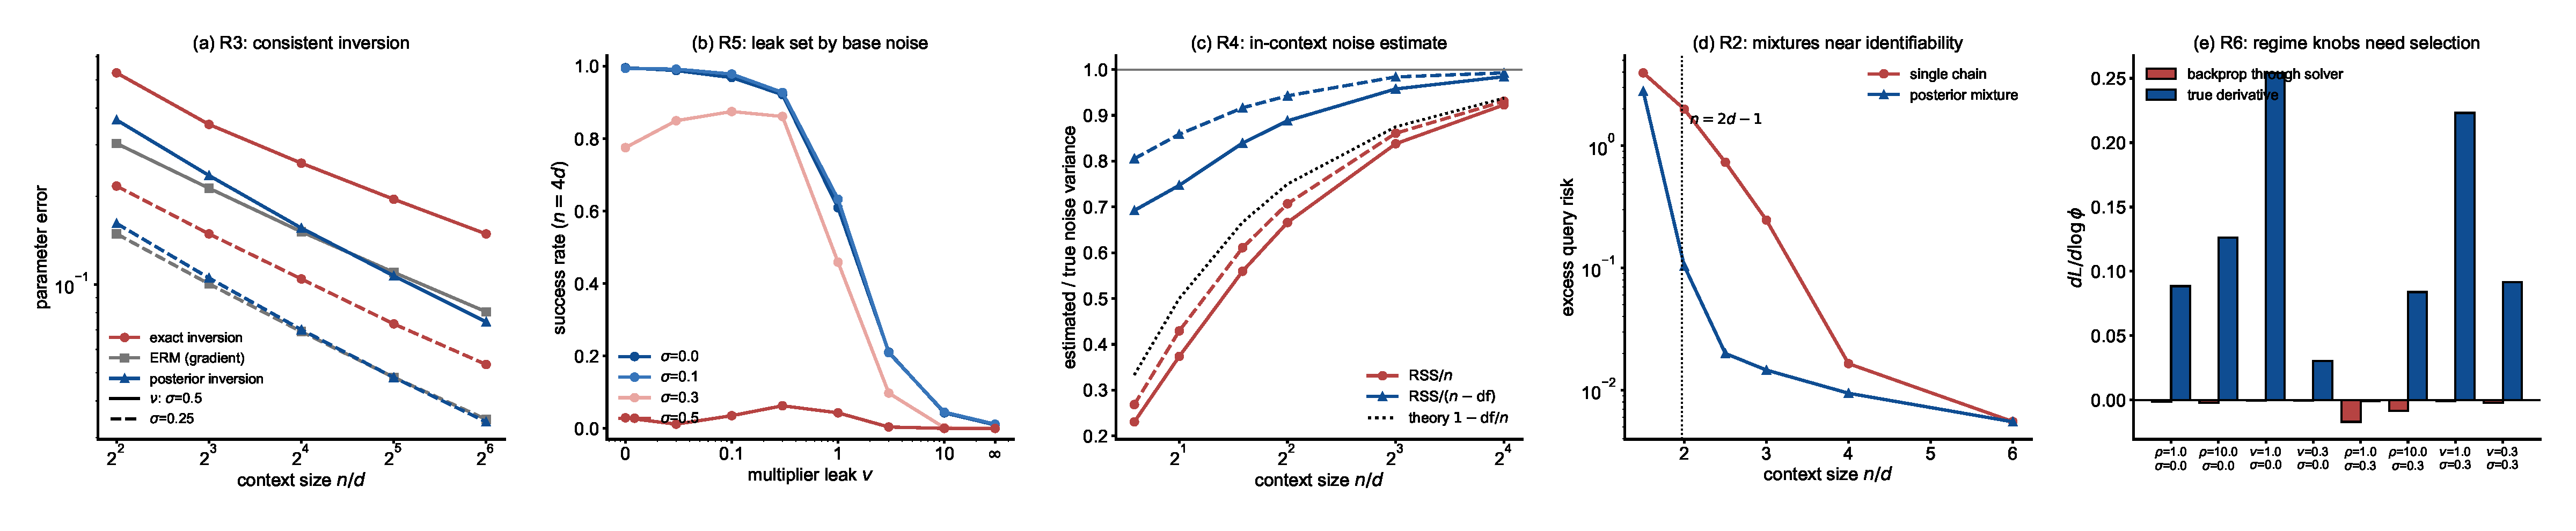
\includegraphics[width=\linewidth]{figures/fig_controlled.pdf}
\caption{\textbf{Learner conditions on controlled bases.}
(a) R3: started at $w^\star$, ERM stationary points move to the norm predicted by Theorem~\ref{thm:l1}(b) ($1.026$ measured vs $\alpha^\star=1.023$ at $\sigma=0.5$, $n=64d$; $1.0045$ vs $1.0032$ at $\sigma=0.25$), exact inversion does not settle, and posterior inversion is consistent ($\|w\|\to1$, error $\propto n^{-1/2}$).
(b) R5: on an exactly decodable base the unleaked multiplier is optimal and success decreases monotonically in the leak ($0.996$ at $v=0$, $0.01$ without multiplier); at $\sigma=0.3$ the optimum moves to $v\in[0.03,0.1]$.
(c) R4: the raw noise estimate follows $1-\dof/n$; the corrected one is within 6\% of the truth for $n\geq4d$.
(d) R2: near $n=2d-1$ a likelihood-weighted mixture of 16 chains lowers excess risk from 1.99 to 0.10 ($n=2d$) and 0.25 to 0.015 ($n=3d$); far above the threshold single chains suffice.
(e) R6: derivative of the outer loss in $\log\rho$ and $\log v$; backpropagation through the solver returns $\approx0$ where the true derivative (central differences on identical tasks) is $+0.03$ to $+0.25$.}
\label{fig:controlled}
\end{figure}

For R3, gradient descent on the ERM started at $w^\star$ reaches $\|w\|=1.0257$ at $\sigma=0.5$, $n=64d$ (theory $1.0232$); posterior inversion stays at $1.002$ and its error falls from $0.365$ ($4d$) to $0.074$ ($64d$), while exact inversion, a Douglas--Rachford iteration on an inconsistent problem \citep{bauschke2017dr}, keeps twice that error.
For R4, at $\sigma=0.5$ the raw estimate is $0.37/0.67/0.84$ of the truth at $n=2d/4d/8d$ (theory $0.50/0.75/0.88$, the gap being the extra freedom of branch choices) and the corrected one $0.75/0.89/0.96$.
For R6, in every configuration the pathwise derivative differs from the true one in sign or by orders of magnitude; with a Gibbs temperature of $0.05$ it reaches $10^4$ in magnitude with random sign.

\section{Real bases}
\label{sec:real}

\paragraph{Bases and tasks.}
\emph{NLP}: 13 attributes of the MRC psycholinguistic database \citep{coltheart1981mrc}; bases GloVe \citep{pennington2014glove} and MiniLM (mean-pooled sentence encoder); pairs of words with $|\Delta\text{attribute}|$; outer training on 7 attributes, deployment on 5 held-out attributes (word-frequency cluster, age of acquisition).
\emph{Graph}: QM9 \citep{ramakrishnan2014qm9} with a 4-layer GINE \citep{hu2020pretraining} pretrained on 14 properties and frozen; deployment on 5 held-out properties.
\emph{CV}: compressive phase retrieval of CIFAR-10 test images \citep{krizhevsky2009cifar} (grayscale $32\times32$) on a 64-dimensional PCA code of the training images, $n\in\{2,3,4,6\}\times64$ Gaussian measurements.
All inner loops share keys ($d=16$ from 64-dim whitened embeddings for NLP/Graph), data, 3000 outer steps and query loss; 1280 (NLP/Graph) or 1024 (CV) held-out sequences per cell, identical across methods.

\begin{table}[t]
\caption{\textbf{Base diagnostics predict the outcome.} $\nu$: mean over deployment tasks of $1-R^2$ of a linear probe from the base; $\flr(\nu)$: Theorem~\ref{thm:b1}; oracle probe: $|\,\text{probe}(a)-\text{probe}(b)|$ trained on all labels; last columns: held-out NMSE at $n=4d$ (CV: $4m$). Selection of the member used training data only.}
\label{tab:bases}
\centering\small
\resizebox{\linewidth}{!}{%
\begin{tabular}{lcccclcc}
\toprule
Base & $\nu$ & $\flr(\nu)$ & oracle probe & R1--R2 & member & self-iteration & best baseline\\
\midrule
synthetic, $\sigma=0$ & 0.00 & 0.00 & 0.00 & yes & exact & \textbf{0.312} & 1.008\\
PCA-64 image code (CV) & 0.026 & 0.065 & 0.067 & yes & $g=1$, $R=8$ & \textbf{0.096} & 0.182\\
synthetic, $\sigma=0.5$ & 0.20 & 0.41 & 0.47 & yes & $g=10$ & \textbf{0.909} & 1.027\\
GINE (Graph) & 0.22 & 0.39 & 0.45 & yes & $g=10$ & \textbf{0.780} & 0.862\\
GloVe (NLP) & 0.29 & 0.53 & 0.57 & yes & $g=10$ & \textbf{0.700} & 0.735\\
MiniLM (NLP) & 0.52 & 0.79 & 1.02 & R1 violated & -- & 0.940 & 0.972\\
synthetic, $\sigma=1$ & 0.51 & 0.78 & 1.03 & R1 violated & -- & 1.002 & 1.011\\
\bottomrule
\end{tabular}}
\end{table}

\begin{figure}[t]
\centering
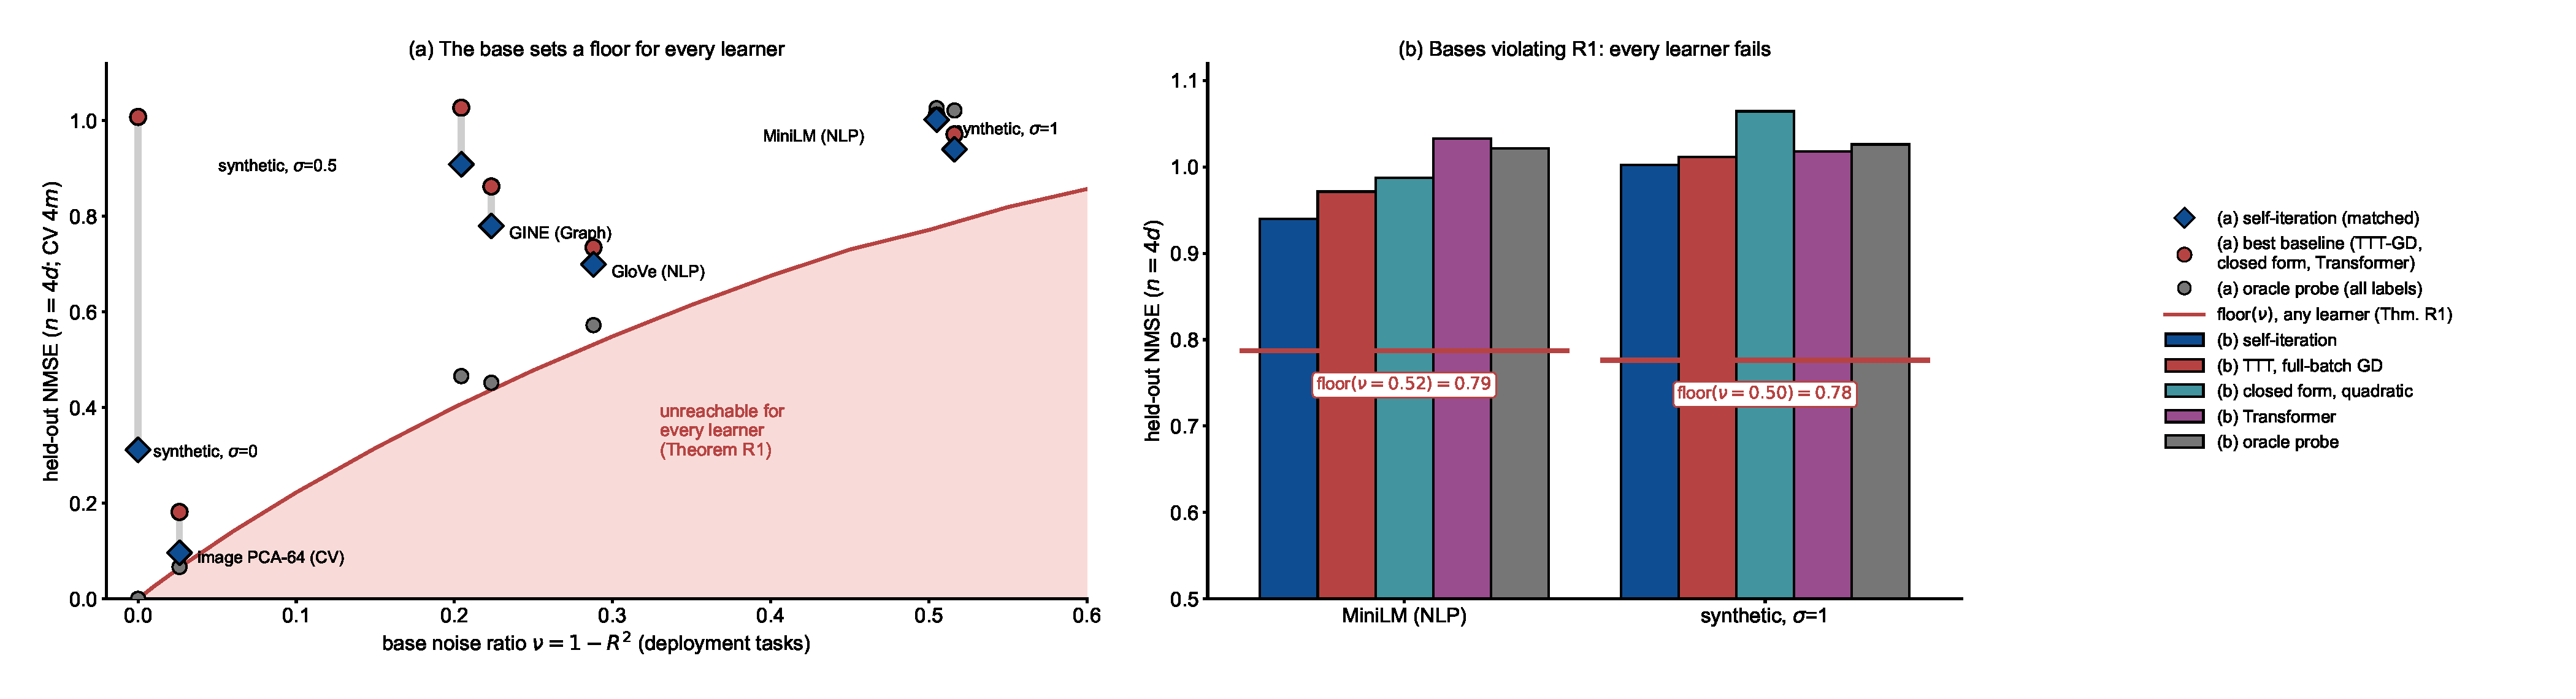
\includegraphics[width=\linewidth]{figures/fig_regime.pdf}
\caption{\textbf{The base decides.} (a) Held-out NMSE against the base noise ratio $\nu$. The shaded region lies below $\flr(\nu)$ and is unreachable for every learner (Theorem~\ref{thm:b1}); the oracle probe sits on the floor. On bases satisfying R1--R2 the matched self-iterating learner (diamonds) is below the best baseline (red). (b) On bases that violate R1, every learner---self-iteration, TTT gradient update, quadratic closed form, Transformer and the oracle probe---stays above the proven floor.}
\label{fig:regime}
\end{figure}

\paragraph{Diagnostics.}
Table~\ref{tab:bases} lists each base's diagnostics.
The measured floors agree with Theorem~\ref{thm:b1}: the oracle probe of every admissible base lies just above $\flr(\nu)$, and for the image code the predicted $\flr(0.026)=0.065$ matches the directly measured error of the true image projected on the code ($0.067$).
GloVe, GINE and the PCA code satisfy R1 and R2 ($n\geq2d$ throughout); MiniLM, with $\nu=0.52$, does not.
On GINE the training properties are nearly exact ($\nu\approx0.01$) while the deployment properties are not ($\nu=0.22$): the regime shift that R6 says backpropagation cannot bridge, and that training-data selection handles.

\begin{figure}[t]
\centering
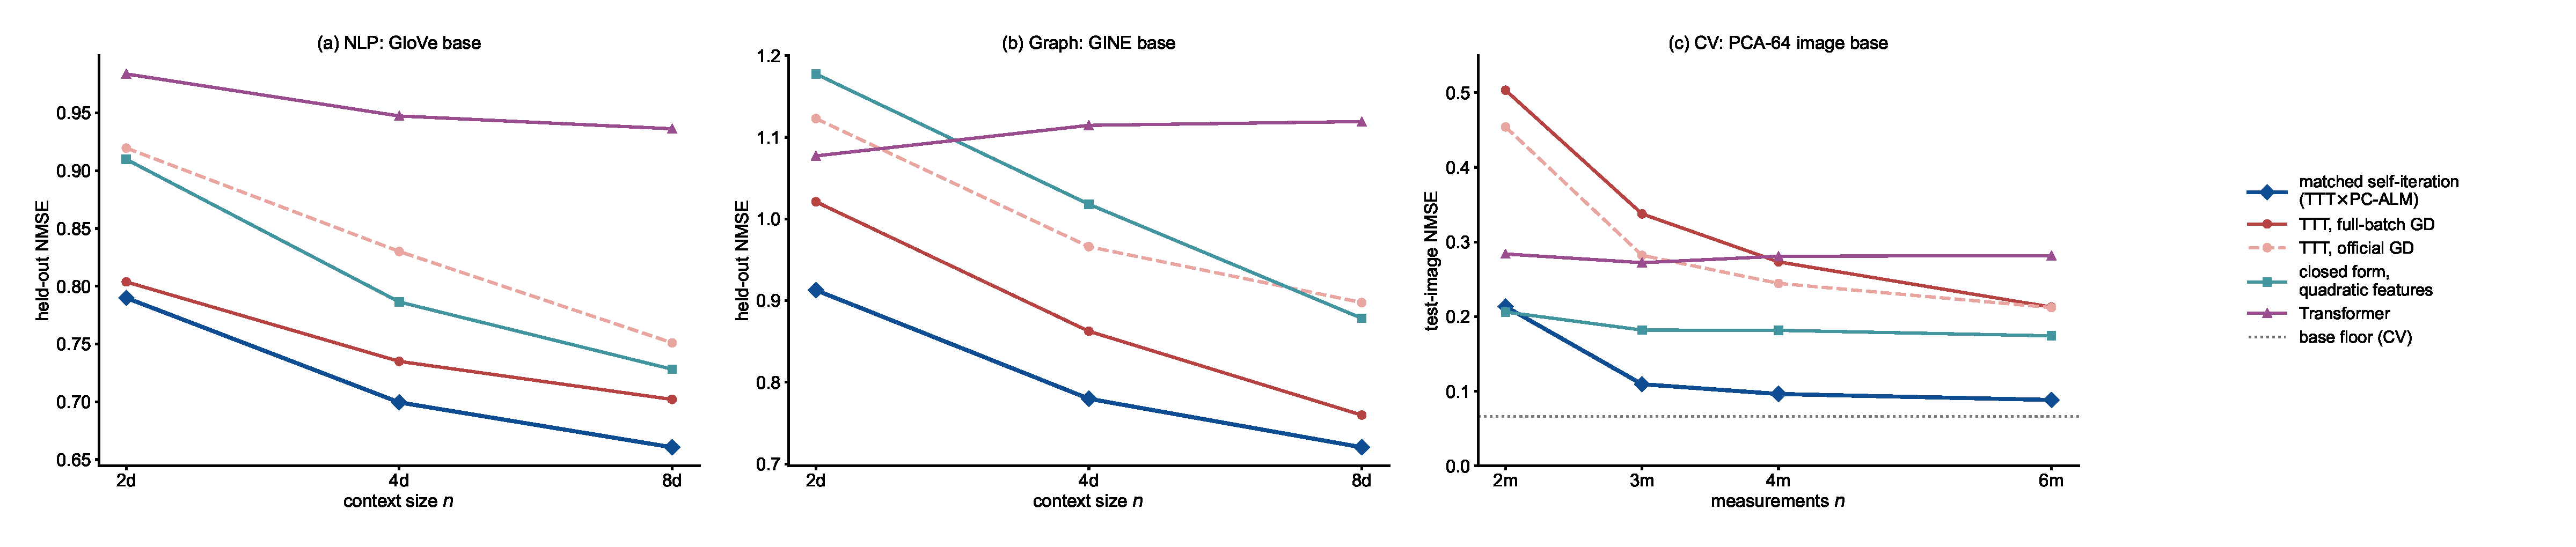
\includegraphics[width=\linewidth]{figures/fig_real.pdf}
\caption{\textbf{Bases that satisfy R1--R2.} Held-out NMSE against context size. NLP and Graph: second seed (new key initialization, training batches and evaluation sequences). CV: test images; dotted line: projection floor of the image code.}
\label{fig:real}
\end{figure}

\begin{table}[t]
\caption{\textbf{Bases that satisfy R1--R2}: held-out NMSE (NLP/Graph at $n=2d/4d/8d$, seed 2; CV at $n=2m/3m/4m/6m$). Paired Wilcoxon tests of self-iteration against each baseline: $p\leq0.034$ in all NLP/Graph cells (all $p<10^{-10}$ except full-batch GD at NLP $2d$), $p<10^{-150}$ for CV at $n\geq3m$; at CV $2m$ the quadratic head ties in mean (difference $+0.007$, 95\% CI $[-0.007,0.023]$) while self-iteration is better on 70\% of images. CV self-iteration entries use $R=8$ likelihood-weighted chains (R2); a single chain gives .761/.177/.102/.089; all baselines are single models. First-seed NLP and Graph values are in Appendix~\ref{app:details}.}
\label{tab:real}
\centering\small
\begin{tabular}{lccc}
\toprule
Inner loop & NLP (GloVe) & Graph (GINE) & CV (PCA-64)\\
\midrule
\textbf{Self-iteration, Algorithm~\ref{alg:learner}} & \textbf{.790/.700/.661} & \textbf{.913/.780/.720} & .213/\textbf{.109}/\textbf{.096}/\textbf{.088}\\
TTT, full-batch GD & .804/.735/.702 & 1.021/.862/.760 & .503/.338/.273/.213\\
TTT, official GD & .920/.830/.751 & 1.123/.966/.898 & .454/.282/.245/.212\\
Closed form, quadratic features & .910/.786/.728 & 1.177/1.018/.878 & \textbf{.206}/.182/.182/.174\\
Closed form, linear ridge & 1.051/1.024/1.015 & 1.055/1.029/1.025 & 2.07/1.54/1.35/1.22\\
Transformer (additional layers) & .984/.947/.936 & 1.077/1.115/1.119 & .284/.272/.281/.282\\
\midrule
$\flr(\nu)$ / oracle probe & .53 / .57 & .39 / .45 & .065 / .067\\
\bottomrule
\end{tabular}
\end{table}

\paragraph{Bases that satisfy R1--R2.}
Table~\ref{tab:real} and Figure~\ref{fig:real}: on every admissible base the self-iterating learner is the best inner loop in every NLP and Graph cell and at every CV context size from $3m$, where it approaches the base floor ($0.088$ vs $0.065$); at $2m$, on the identifiability threshold, it ties the quadratic closed form in mean.
The margin over TTT's full-batch gradient update is $0.035$--$0.041$ on NLP ($4d$, $8d$) and $0.04$--$0.11$ on Graph, and over the quadratic closed form $0.07$--$0.26$.
The first seed gives the same ordering (Appendix~\ref{app:details}).
The member selected on training data (Table~\ref{tab:bases}) is the one Theorems~\ref{thm:l1}--\ref{thm:l2} predict from $\nu$: the exact member for $\nu=0$, a weak leak for the nearly exact image code, a strong leak for $\nu\approx0.2$--$0.3$; in each case it was also the best member on held-out data (Appendix~\ref{app:details}).

\paragraph{A base that violates R1.}
On MiniLM ($\nu=0.52$, $\flr=0.79$) and on the synthetic base with $\sigma=1$ ($\nu=0.51$, $\flr=0.78$) every learner stays above the floor: self-iteration $0.94$/$1.00$, TTT gradient update $0.97$/$1.01$, quadratic closed form $0.99$/$1.06$, Transformer $1.03$/$1.02$ and even the oracle probe trained on all labels $1.02$/$1.03$ (Figure~\ref{fig:regime}b).
This is the failure Theorem~\ref{thm:b1} proves for every learner; it is a property of the base.

\section{Related work}

\paragraph{Test-time training and in-context learning.}
TTT layers \citep{sun2023ttt,sun2024ttt}, fast weights \citep{schlag2021fastweights} and test-time regression \citep{wang2026ttr} define the inner-loop design space; Transformers can implement gradient-like in-context learners \citep{garg2022icl,vonoswald2023icl}. We characterize which bases admit an iterating nonlinear inner loop and what that loop must satisfy.
\paragraph{Meta-learning through inner solvers.}
MAML \citep{finn2017maml} and differentiable closed-form solvers \citep{bertinetto2019r2d2} backpropagate through inner learners; Theorem~\ref{thm:l5} identifies the boundary term that pathwise gradients miss for branch-controlling knobs \citep[cf.][]{mohamed2020mcgrad}.
\paragraph{Predictive coding, lifting and ALM.}
Predictive coding \citep{whittington2017predictive} and PC-ALM \citep{seely2026pcalm} introduce activities and multipliers; lifted, MAC and ADMM training decouple layers \citep{carreira2014mac,taylor2016admm,askari2018lifted}; ALM and proximal methods are classical \citep{hestenes1969multiplier,rockafellar1976augmented}.
\paragraph{Phase retrieval and single-index learning.}
HIO/DR/RAAR \citep{fienup1982phase,bauschke2002phase}, Wirtinger flow \citep{candes2015wf} and AMP \citep{rangan2011gamp} solve multi-branch problems; injectivity needs $2d-1$ real measurements \citep{balan2006phase}. Single-index theory separates correlational and data-reuse algorithms \citep{benarous2021online,damian2023smoothing,dandi2024reuse,lee2024neural}. EM \citep{dempster1977em} underlies R3 and degrees-of-freedom corrections \citep{craven1979gcv} underlie R4.

\section{Scope and conclusion}

Our bases are frozen encoders with a trained projection, the relations are pair differences and simulated measurements of real images, and the models are small; Theorem~\ref{thm:b1} assumes the Gaussian residual model \eqref{eq:model}, Theorem~\ref{thm:l2}(c) a fixed branch assignment, and Theorem~\ref{thm:l5} smoothly moving branch boundaries.

Inference-time self-iteration earns its compute on multi-branch relations, where gradient, closed-form and additional-layer inner loops cannot follow.
Whether a pretrained model can use it is decided by the base: its undecodable fraction sets a floor no learner can pass, its keys must cover the deployment directions, and its task dimension must fit the context.
On a base that meets these conditions, a self-iterating learner that is consistent under the base's residual noise, leaks its multipliers accordingly, corrects its noise estimates, mixes near identifiability and selects its branch-controlling knobs on data, is the best inner loop across language, molecular and image bases.

\subsection*{Reproducibility statement}
An anonymized archive with the code, the exact configuration of every run, the per-sequence result files and the figure scripts is provided as supplementary material; its README maps each table and figure to the script and result files that produce it. Every number in the paper is read from a saved result file, and all figures are regenerated from the raw result files. Section~\ref{sec:real} and Appendix~\ref{app:details} give data sources, splits, seeds and hyper-parameters. Member selection used training data only; evaluation sequences are fixed by seed and identical across models, which makes the paired tests valid.

\subsection*{AI use statement}
In this work, we used generative AI tools for two purposes: to polish the writing, and to create the figures.
All figures were drawn by coding agents (Claude Code and Codex) following figure-making skills, i.e., instruction files that fix the house style, the panel layout and automatic legibility checks.
Each figure is produced by a matplotlib script that reads the archived experimental outputs; no image-generation model was used.
We have reviewed all AI-assisted work.
We take responsibility for the final content of this work, including text, claims or artifacts produced with the aid of generative AI.

\bibliography{references}
\bibliographystyle{iclr2027_conference}

\appendix

\section{Proofs}
\label{app:proofs}

\subsection{Theorem~\ref{thm:b1}}
(a) The query label $y_q$ is conditionally independent of the context given $(m_q,u)$, because query items are fresh. For any learner $\hat y_q=h(k_q,D)$, the law of total variance gives $\Ex(y_q-\hat y_q)^2\geq\Ex\,\mathrm{Var}(y_q\mid k_q,D)\geq\Ex\,\mathrm{Var}(y_q\mid k_q,D,u)=\Ex\,\mathrm{Var}(y_q\mid m_q)$. For $y=|m+e|$ with $e\sim\mathcal N(0,\sigma^2)$, $\Ex[y^2\mid m]=m^2+\sigma^2$ and $\Ex[y\mid m]=\Fsig(m)$; since $y$ is non-degenerate given $m$, $\mathrm{Var}(y\mid m)>0$. Dividing by $\mathrm{Var}(y)=2-\tfrac{4}{\pi}$ (for $m+e\sim\mathcal N(0,2)$) gives the floor, which is 0 at $\nu=0$ and 1 at $\nu=1$; the listed values are Monte Carlo evaluations with $4\times10^5$ samples.
(b) By the chain rule $I(u;D)=\sum_iI(u;y_i\mid k_i,y_{<i})\leq\sum_iI(m_i;y_i\mid k_i)$, since given $k_i$, $u\to m_i\to y_i$ is Markov and $y_i$ is independent of $y_{<i}$ given $m_i$. As $y_i=|m_i+e_i|$ is a function of $m_i+e_i$, data processing gives $I(m_i;y_i\mid k_i)\leq I(m_i;m_i+e_i\mid k_i)\leq\tfrac12\log(1+\mathrm{Var}(m_i)/\mathrm{Var}(e_i))=\tfrac12\log(1/\nu)$ by the Gaussian channel capacity. Fano's inequality over a $\delta$-packing of size $M\geq\delta^{-(d-1)}$ gives $(1-P_e)\log M-\log2\leq I(u;D)$. The folded-channel values for Gaussian $m$ follow from $h(y)=\tfrac12\log(4\pi e)-\log2$ and a Monte Carlo evaluation of $h(y\mid m)$.

\subsection{Corollary~\ref{cor:b2}}
With $x\sim\mathcal N(0,I)$ and $P$ an orthogonal projection, $u^\top x=u_\parallel^\top x+u_\perp^\top x$ where $u_\perp^\top x$ is independent of $Px$. For a learner that sees only $Px$, $u_\perp^\top x$ is indistinguishable from the base residual, so the undecodable variance is $\nu+(1-\nu)\|u_\perp\|^2/\|u\|^2$ of the attribute variance and Theorem~\ref{thm:b1} applies.

\subsection{Proposition~\ref{prop:b3}}
(a) For a fixed sign pattern $b$, noiseless consistency means $Kw=b\odot y$, whose solution set is empty or an affine subspace of dimension $d-\mathrm{rank}K\geq d-n$. Under a prior with a density the posterior then has positive variance along this subspace, so $k_q^\top w$ has positive posterior variance for almost every $k_q$, and every predictor has positive excess risk. Quantitatively, reveal the signs, so that the context determines $Ku$ exactly; a learner with less information cannot do better. With $u\sim\mathcal N(0,d^{-1}I)$ the posterior of $m_q=k_q^\top u$ is $\mathcal N(\mu_q,v_q)$ with $v_q=\|P_\perp k_q\|^2/d$, $P_\perp$ the projection onto the null space of $K$, so $\E v_q=(d-n)/d$. The variance of a folded normal $|\mathcal N(\mu,v)|$ is minimized at $\mu=0$, where it equals $(1-2/\pi)v$; hence $\E\,\mathrm{Var}(y_q\mid D,\text{signs})\geq(1-2/\pi)(d-n)/d$, while $\mathrm{Var}(y_q)=(1-2/\pi)\E m_q^2=1-2/\pi$. Dividing gives $\mathrm{NMSE}\geq1-n/d$. (b) is the complement-property characterization of \citet{balan2006phase}.

\subsection{Theorem~\ref{thm:features}}
\label{app:features}
For $f_u(x)=g(u^\top x)$ and Gaussian $x$, $\langle f_u,f_v\rangle=(u^\top v)^3$. The covariance operator $\Ex_uf_u\otimes f_u$ has the nonzero spectrum of the kernel $(u^\top v)^3$ on the sphere, which the Funk--Hecke formula diagonalizes in spherical harmonics; $t^3$ has Gegenbauer components of degrees 1 and 3 only. The degree-1 eigenvalue is $3/(d(d+2))$ (multiplicity $d$) and, since the trace is 1, the degree-3 eigenvalue is $(d-1)/((d+2)N_3)$ (multiplicity $N_3$). The best $M$-dimensional $u$-independent approximation leaves at least the eigenvalues outside the top $M$.

\subsection{Multiplier escape and Theorem~\ref{thm:l2}(b)}
\label{app:escape}
While the primal stays at $z_0$ with residual $r_0$, the multiplier accumulates $\lambda_t=\rho r_0\sum_{j=1}^t\beta^j$ with $\beta=(1+\rho v)^{-1}$ ($\lambda_t=t\rho r_0$ for $v=0$). Block energies are affine in $\lambda$ at fixed primal states, so the gap to a legal competitor $z'$ is $\Delta-\kappa c_t$ with $\kappa=-r_0^\top(r(z')-r_0)$ in the block normalization. For $v>0$, $c_t\uparrow\rho\beta/(1-\beta)=1/v$.

\subsection{Theorem~\ref{thm:l1}}
(a) At a fixed point with $v=0$, $s=Kw$. The activity step's first-order condition at $s_i\neq0$ is $\ell'(s_i)+\lambda_i=0$, i.e.\ $\lambda_i=-2(|k_i^\top w|-y_i)\sgnx(k_i^\top w)$, and the parameter step gives $\mu w=K^\top\lambda/\rho$. Together, $\sum_i2(|k_i^\top w|-y_i)\sgnx(k_i^\top w)k_i+\rho\mu w=0$.
(b) $e$ takes both signs with positive probability, so $\Fsig(m)>|m|$ strictly. Conditioning on $k$, $\nabla R(w^\star)=2\Ex[(|m|-\Fsig(m))\sgnx(m)k]$; writing $k=mw^\star+k_\perp$ with $k_\perp$ centered and independent of $m$, $\nabla R(w^\star)=-2c_\sigma w^\star$. On the ray, $R(\alpha w^\star)=\alpha^2-2\alpha(1+c_\sigma)+\Ex y^2$.
(c) $\Ex[y\mid k]=\Fsig(m)$ and $\Fsig(0)=\Ex|e|$.
(d) For $s\sim\mathcal N(m,\sigma^2)$, $\Pr(s>0\mid|s|=y)=(1+e^{-2ym/\sigma^2})^{-1}$, hence $\Ex[s\mid|s|=y]=T_{\sigma^2}(y,m)$ and $\Ex[T_{\sigma^2}(y,m)\mid k]=\Ex[s\mid k]=m$. As $\tau\to0$, $\Ex[T_\tau\mid k]\to\sgnx(m)\Fsig(m)\neq m$.
Gibbs activity: the branch minimizers are $s_\pm=(\pm2y+\rho a)/(2+\rho)$ with values $\tfrac{\rho}{2+\rho}(y\mp a)^2$, whose difference is $\tfrac{4\rho ya}{2+\rho}$.

\subsection{Theorem~\ref{thm:l2}}
(a) For $v>0$ the fixed-point multiplier is $\lambda=r/v$ with $r=s-Kw$; the parameter step gives $\mu w=K^\top r(1+\tfrac{1}{\rho v})$; on the selected branch, $2(s_i-b_iy_i)+\rho r_i+\lambda_i=0$ gives $r_i=-2(k_i^\top w-b_iy_i)/(2+\rho+1/v)$. Hence $\mu w=-2c\sum_ik_i(k_i^\top w-b_iy_i)$ with $c=\tfrac{1+\rho v}{\rho(1+\rho v+2v)}$, the normal equation of the stated ridge problem with $\mu_v=\mu/(2c)$. Conversely every self-consistent $(b,w)$ defines $r$, $\lambda=r/v$, $s=Kw+r$ fixed by the three updates; $v=0$ is Theorem~\ref{thm:l1}(a).
(c) With $t=Kw^\star+\xi$, $w^\star\sim\mathcal N(0,d^{-1}I)$, $\xi\sim\mathcal N(0,\sigma^2I)$, the posterior mean $(K^\top K+d\sigma^2I)^{-1}K^\top t$ minimizes the MSE among all estimators.

\subsection{Propositions~\ref{prop:l3} and \ref{prop:l4}}
R4: $\Ex\|(I-H)t\|^2=\|(I-H)Kw^\star\|^2+\sigma^2\mathrm{tr}((I-H)^2)$; for $\mu\to0$, $H$ is a rank-$d$ projection. $\mathrm{tr}H=\sum_j\eta_j/(\eta_j+\mu)$ decreases in $\mu$, $2h-h^2$ increases on $[0,1]$ and $\mu_v$ increases in $v$, giving the feedback.
R2: for any predictor $a$, $\Ex[(y-a)^2\mid k,D]-\Ex[(y-\hat y_B)^2\mid k,D]=(a-\hat y_B)^2$ with $\hat y_B=\pi F_1+(1-\pi)F_2$. If $w_1\neq\pm w_2$, $|k^\top w_1|=|k^\top w_2|$ only on two hyperplanes.

\subsection{Theorem~\ref{thm:l5}}
Write $L(\phi)=\sum_B\int_{\Omega_B(\phi)}\ell_B(\phi,D)p(D)dD$ with smooth $\ell_B$; Reynolds' transport theorem gives the interior term plus boundary integrals, which combine across adjacent regions into the jump term. Backpropagation differentiates $\ell_B$ at a fixed pattern $B$ and returns only the interior term. With a Gibbs temperature, the branch weight $\sigma((F_--F_+)/\tau)$ has derivative $O(1/\tau)$ in a band of width $O(\tau)$. For $v=g\hat r^2$, $\partial\lambda_{t+1}/\partial g=-\rho\hat r_t^2(\lambda_t+\rho r_t)/(1+\rho g\hat r_t^2)^2$.

\section{PC-ALM as proximal Douglas--Rachford}
\label{app:dr}
With $u=\lambda/\rho$, $a=Kw-u$, $h$ the sum of local losses and $C=\mathrm{range}(K)$, fixed $\rho$, exact proximal steps, $\mu\to0$ and the multiplier updated before the parameter, eliminating $\lambda$ gives $S=\mathrm{prox}_{h/\rho}(a)$ and $a^+=a+P_C(2S-a)-S$.

\section{Experimental details}
\label{app:details}
\paragraph{Controlled bases.} $d=32$, 512 tasks per cell, float64, 300--400 inner iterations (2000 gradient steps for the ERM), success = overlap $>0.95$, excess risk relative to $\Fsig(k^\top w^\star)$ normalized by the query variance; finite differences with steps $0.05$ and $0.2$ in $\log\phi$ on 2048 identical tasks.
\paragraph{Real bases.} 64-dim PCA-whitened embeddings, $d=16$ keys; Adam ($3\cdot10^{-3}$, batch 64, 3000 steps; CV batch 32, 1000 steps for fixed-code models); $T=30$ inner iterations (CV $T=100$, $R=8$). Base diagnostics: ridge probe on 80\% of items, $R^2$ on the rest. Deployment attributes were chosen from decodability alone.
\paragraph{Member selection on training data.} Training-attribute NMSE for exact/$g{=}1$/$g{=}10$ members: NLP 0.977/0.861/0.847; Graph (median over properties) 0.157/0.146/0.065; synthetic $\sigma=0$ 0.066/0.381/0.092; training-image NMSE for CV at $2m$ 0.989/0.210/0.582. The selected member was the best on held-out data in every domain.
\paragraph{First seed.} NLP ($2d/4d/8d$): self-iteration .809/.711/.674, full-batch GD .811/.752/.708, official GD .927/.840/.759, quadratic .877/.771/.727, Transformer .986/.953/.922. Graph: .867/.742/.688, 1.010/.871/.783, 1.078/1.009/.987, 1.162/1.029/.902, 1.097/1.146/1.166.

\end{document}
